\subsection{Besonderheiten der FM-Synthese}
\FloatBarrier
\subsubsection{Phasenmodulation als FM}
Frequenzmodulation (FM) und Phasenmodulation (PM) können unter dem Oberbegriff Winkelmodulation zusammen gefasst werden. Im Folgenden soll der Zusammenhang zwischen PM und FM genauer beschrieben werden. Zuerst wird die mathematische Herleitung der beiden Modulationen beschrieben. Anschließend wird die Ähnlichkeit der beiden Verfahren erörtert und im Kontext der Akustik beschrieben. Interessanterweise führte die Publikation von Chowning zu anfänglicher Verwirrung, da er in seinem Artikel eine Formel beschreibt, die einer PM gleicht und ein MUSIC V Patch der eine FM beschreibt. \cite{rossum1999method} Des Weiteren kann dem Yamaha Patent für die Implementierung eines FM-Synthesizer entnommen werden, dass Yamaha ihre FM-Synthese über eine PM erzeugte. \cite{oya1987electronic} 

Wie der Name Winkelmodulation andeutet, wird der Phasenwinkel eines Trägersignales in Abhängigkeit eines Modulationssignals verändert. Die Amplitude \(A\) bleibt während der Modulation konstant. In der allgemeinsten Form kann ein winkelmoduliertes Signal als Sinusfunktion eines sich zeitlich ändernden Winkels beschrieben werden:
\begin{equation}
s(t)=A*sin(\theta(t))
\label{eq:signal_basis_funktion}
\end{equation}
Dabei wird \(\theta(t)\) als \textit{momentaner Winkel} bezeichnet und ist als Summe der konstanten Kreisfrequenz $\omega_0$ multipliziert mit der Zeit $t$ und der \textit{momentanen Phase} $\varphi(t)$ definiert:
\begin{equation*}
\theta(t)=\omega_0t + \varphi(t)
\end{equation*}

Wird nun die momentane \textbf{Phase} des Trägersignals proportional zum Modulationssignal \(p(t)\) verändert, erhält man das \textbf{phasenmodulierte} Signal \(s_{PM}(t)\). \cite[S. 209]{lathi}
Für die momentane Phase ergibt sich folgende einfache Formel:
\begin{equation}
\varphi(t)=\varphi_0+k_{PM}*p(t)
\label{eq:varphi_t}
\end{equation}
Für akustische Anwendungen wird der konstante Teil \(\varphi_0\) der Phase nicht benötigt und wird als 0 angenommen. Bei \(k_{PM}\) handelt es sich um eine Proportionalitätskonstante, welche Modulatorkonstante genannt wird. Die Modulatorkonstante bestimmt, wie stark das Modulationssignal auf das Trägersignal einwirkt. Wird nun \(\theta(t)\) in die allgemeine Formel~\ref{eq:signal_basis_funktion} für ein moduliertes Signal substituiert und das obige \(\varphi(t)\) eingesetzt, ergibt sich die Formel für das phasenmodulierte Signal:
\begin{equation}
s_{PM}(t)=A*sin(\omega_0t + \varphi(t))=A*sin(\omega_0t+k_{PM}*p(t))
\label{eq:s_pm}
\end{equation}
Für die Herleitung der Frequenzmodulation muss zuvor noch der Begriff der \textit{momentan Kreisfrequenz} \(\omega_m(t)\) eingeführt werden.
Diese entspricht der Änderung des Phasenwinkels in Abhängigkeit der Zeit. Daher kann die momentan Kreisfrequenz durch die erste Ableitung des Phasenwinkels nach der Zeit $\dot \theta(t)$ bestimmt werden. \cite[S. 209]{lathi}
\begin{equation}
\omega_m(t)=\dot \theta(t)=\frac{d\theta(t)}{dt}=\frac{d[\omega_0t+\varphi(t)]}{dt}=\frac{d\omega_0t}{dt}+\frac{d\varphi(t)}{dt}=\omega_0+\frac{d\varphi(t)}{dt}
\label{eq:omega_m_herleitung}
\end{equation}
Wieso dieser Zusammenhang gültig ist, lässt sich einfach veranschaulichen. Bei \(\omega_m\) handelt es sich um die Kreisfrequenz, also wie häufig eine Schwingung einen Kreis pro Zeitspanne durchläuft, hier in Sekunden. Bei einer Kreisfrequenz von \(\omega=2 s^{-1}\) wird ein Phasenwinkel von \(4\pi\) pro Sekunde überstrichen. Wird nun die Kreisfrequenz erhöht, wird ein größerer Phasenwinkel überstrichen. Daher gibt die momentane Kreisfrequenz die Änderungsrate des momentanen Phasenwinkels zu einem bestimmten Zeitpunkt \(t\) an. Da die Änderung einer Funktion der Ableitung dieser Funktion entspricht, ergibt sich der Zusammenhang aus der obigen Formel. Eine Analogie aus der Physik hierzu ist der Zusammenhang zwischen Weg \(s(t)\) und Geschwindigkeit \(v(t)\). Die Geschwindigkeit gibt die Änderung des Weges pro Zeiteinheit vor und somit gilt, \(\dot{s(t)}=v(t)\). In unserem Zusammenhang verhält sich die Kreisfrequenz analog zur Geschwindigkeit und der Phasenwinkel ist im Prinzip die Strecke ausgedrückt als Winkel.

Wird die momentane \textbf{Frequenz} des Trägersignals proportional zum Modulationssignal \(f(t)\) verändert, erhält man das \textbf{frequenzmodulierte} Signal \(s_{FM}(t)\). \cite[S. 210]{lathi} Für die momentane Frequenz ergibt sich analog zur Phasenmodulation folgende Formel:
\begin{equation}
\omega_m(t)=\omega_0+k_{FM}*f(t)
\label{eq:omega_m}
\end{equation}

Bei \(k_{FM}\) handelt es sich wieder um eine Modulatorkonstante und gibt an wie stark das Modulationssignal das Trägersignal beeinflusst. Um nun das frequenzmodulierte Signal zu erhalten muss die momentan Frequenz, analog wie bei der Phasenmodulation, in \(s(t)\) eingesetzt werden. Jedoch kommt \(\omega_m\) nicht direkt in \(s(t)\) oder \(\theta(t)\) vor. Aus Formel~\ref{eq:omega_m_herleitung} ist bekannt, dass die momentane Frequenz gleich der ersten Ableitung des momentan Winkels \(\theta(t)\) ist. Im Umkehrschluss bedeutet das, dass die Integration von \(\omega_m\) nach der Zeit gleich \(\theta(t)\) sein muss.
\begin{equation*}
\theta(t)=\int_0^t{\omega_m(t)} dt = \int_0^t{\omega_0 + k_{FM}*f(t)} dt = \omega_0t + k_{FM} * \int_0^t{f(t)} dt
\end{equation*}
Setzt man diesen Term in \(s(t)\) ein, erhält man die Formel für ein frequenzmoduliertes Signal
\begin{equation}
s_{FM}(t)=A*sin(\omega_0t + k_{FM} * \int_0^t{f(t)} dt)
\label{eq:s_fm}
\end{equation}
Es sei angemerkt, dass wissentlich die Integrationskonstante mit Null gleichgesetzt wurde und somit nicht in den Formeln auftritt, da sie für unsere Beobachtungen unerheblich ist und die Terme nur unnötig verkomplizieren würde.

Wie einführlich erklärt, ist die Phasenmodulation mit der Frequenzmodulation verwandt. Wie ähnlich die beiden Verfahren sind, ist leicht ersichtlich an den Formeln für die modulierten Signalen~\ref{eq:s_pm} und \ref{eq:s_fm}. Beide Formeln sind bis auf die letzte Addition gleich. Daraus lässt sich eine Bedingung ableiten, welche beschreibt wann eine FM durch eine PM oder umgekehrt dargestellt werden kann. Dies ist genau dann möglich, wenn die Signale \(s_{PM}(t)\) und \(s_{FM}(t)\) gleich sind. Daraus ergibt sich für die Modulationssignale \(p(t)\) und \(f(t)\) folgende Beziehung:
\begin{equation}
k_{PM}*p(t)=k_{FM} * \int_0^t{f(t)} dt
\end{equation}

Vorausgesetzt \(k_{PM}\) ist gleich \(k_{FM}\), dann können beide Faktoren aus der Gleichung eliminiert werden. Ist es nun möglich, für \(f(t)\) eine Ableitung zu finden, kann eine PM durch eine FM dargestellt werden. Durch die Ableitung von \(\int{f(t)}\) wird das Integral aufgehoben und die Gleichung reduziert sich zu einem einfachen \(p(t)=f(t)\). Umgekehrt gilt, dass genau dann eine FM durch eine PM dargestellt werden kann, wenn \(p(t)\) integrierbar ist. Unter diesen Bedingungen sind beide Verfahren mathematisch betrachtet gleich. Daher kann nur anhand der Betrachtung eines modulierten Signals nicht darauf zurück geschlossen werden, ob es mit einer Phasen- oder Frequenzmodulation moduliert wurde. Die unterschiedlichen Namen (FM, PM) zeigen somit nur, welche Größe des Modulationssignals (\(f(t), p(t)\)) proportional ist. \cite[S. 210]{lathi}
Eine weitere, erwähnenswerte Eigenschaft lässt sich gewinnen, wenn der momentane Phasenwinkel beider Verfahren gegenüber gestellt wird. Während \(\varphi(t)\) für PM durch die Formel~\ref{eq:varphi_t} gegeben ist, muss \(\varphi(t)\) für FM durch gleichsetzten der Formeln~\ref{eq:omega_m_herleitung} und \ref{eq:omega_m} gewonnen werden:
\begin{eqnarray*}
\omega_0+\frac{d\varphi(t)}{dt}&=&\omega_0+k_{FM}*f(t) \\
\frac{d\varphi(t)}{dt}&=&k_{FM}*f(t)
\end{eqnarray*}
Draus ergibt sich für ein gemeinsames Modulationssignal \(m(t)\) folgender Zusammenhang:
\begin{center}
\fbox{\parbox{7.5cm} { 
	\begin{eqnarray*}
	\varphi(t)&=&k_{PM}*m(t) : \textbf{PM} \\
	\frac{d\varphi(t)}{dt}&=&k_{FM}*m(t) : \textbf{FM}
	\end{eqnarray*}
}}
\end{center}
Da \({d\varphi(t)}/{dt}\) die Ableitung und somit die Änderung von \(\varphi(t)\) ist, ändert sich \(\varphi(t)\) wenn die Ableitung sich ändert und umgekehrt. PM und FM treten also immer gleichzeitig auf.

Bisher wurde nur das modulierte Signal betrachtet und dessen Abhängigkeit von den allgemeinen Modulationssignalen \(p(t)\) bzw. \(f(t)\). Für die bisherigen Erkenntnisse war es einfach nicht notwendig, sich auf eine spezifische Modulationssignale festzulegen. Diese allgemeine Betrachtung ist jedoch mehr für die Nachrichtentechnik interessant als für einen FM-Synthesizer.
Daher werden die folgenden Formeln im Kontext der Akustik betrachtet und weniger streng mathematisch wie bisher. So kann zum Beispiel das menschliche Gehör keine initiale Phasenverschiebungen wahrnehmen. Dies erlaubt Umformungen von Termen, die mathematisch nicht korrekt sind, jedoch am Ergebnis, also dem hörbaren Klang, keine Auswirkung haben. Deshalb ist es auch korrekt, bei den obigen Umformungen den initialen Phasenwinkel $\varphi_0$ zu ignorieren. Des Weiteren wird im Folgenden ein sinusförmiges Signal als Modulator verwendet, welches sowohl für die PM als auch die FM verwendet wird und wie folgt definiert ist:
\begin{equation}
m(t)=f(t)=p(t)=sin(\omega_m t)
\end{equation}
Wobei \(\omega_m\) die Modulationskreisfrequenz darstellt. Eingesetzt in die Formeln für PM und FM ergibt sich
\begin{eqnarray*}
s_{PM}(t)&=&A*sin(\omega_0t+k_{PM}*sin(\omega_m t)) \\
s_{FM}(t)&=&A*sin(\omega_0t+k_{FM}*\int_0^t{sin(\omega_m t)} dt)
\end{eqnarray*}
Die von Chowning vorgestellte Formel gleicht der Formel für eine PM, \cite{chowningPaper} wobei Chowning seine Formel als Frequenzmodulation vorstellt. Wieso diese Aussage trotzdem korrekt ist, wird im Folgenden gezeigt. Im ersten Schritt muss das Integral innerhalb von \(s_{FM}\) ausgerechnet werden:
\begin{equation*}
s_{FM}(t)=A*sin(\omega_0t-\frac{k_{FM}}{\omega_m}*cos(\omega_m t))
\end{equation*}
Mathematisch gesehen, unterscheidet sich diese Formel zu einer Phasenmodulation. Genauer gesagt, ergibt sich durch die Integration eine Verschiebung von einer Phase, da ein negativer Kosinus genau eine Phase verschoben zu einem Sinus ist. Wie bereits erwähnt, nimmt das Gehör jedoch keine initiale Phasenverschiebungen wahr. Unter dieser Annahme, kann der negative Kosinus mit einem positiven Sinus ausgetauscht werden, ohne eine hörbare Veränderung des Tons zu erzeugen.
\begin{equation*}
e(t)=A*sin(\omega_0t+\frac{k_{FM}}{\omega_m}*sin(\omega_m t))
\end{equation*}
Die dadurch gewonnene Formel ähnelt in der Struktur der von Chowning vorgestellten Formel schon sehr. Jedoch ist in der obigen Formel der Modulationsindex $I$ nicht direkt ersichtlich. Dieser ist bei Chowning als $I=d/\beta$ definiert. Wobei $d$ dem Frequenzhub entspricht und $\beta$ der Modulationsfrequenz $\omega_m$ (s. Kapitel~\ref{chowningparameter}). Für den Frequenzhub $\Delta f$ gilt: \cite[S. 219]{lathi}
\begin{equation*}
\Delta f = k_{FM}*[\dot f(t)]_{\max}
\end{equation*}
Da unser $f(t)$ eine Sinusfunktion darstellt, entspricht die Ableitung $\dot f(t)$ einer Kosinusfunktion und somit ist ihr Maximum gleich $1$ und entfällt in der obigen Formel. Somit reduziert sich der Frequenzhub zu $\Delta f=k_{FM}$ und kann in die obige Formel eingesetzt werden. Dadurch kann nun $\Delta f / \omega_m$ durch den Modulationsindex $I$ substituiert werden und es ergibt sich die originale Formel nach Chowning:
\begin{equation}
e(t)=A*sin(\omega_0t+I*sin(\omega_m t))
\label{eq:FM_Chowning}
\end{equation}
Diese Formel entspricht somit der von Chowning vorgestellten Formel für eine FM-Synthese und ist im Kontext der Akustik korrekt.



\FloatBarrier
\subsubsection{Seitenfrequenzbänder (Evtl. Besselfunktion)}
\label{bulli:ohrToeneUndFrequenzen}
Ein Ton wird durch eine einfache Sinusschwingung erzeugt. Die Tonstärke, also die Lautstärke eines Tones, hängt von der Amplitude der Schwingung ab. Je größer die Amplitude desto lauter wirkt der Ton. Die Frequenz einer Schwingung empfindet der Mensch als Tonhöhe. Je größer die Frequenz der Schwingung desto höher wird der Ton empfunden. 
Ein natürlicher Klang setzt sich nicht aus einer einzigen Frequenz zusammen, sondern aus mehreren Teiltönen. Jeder Teilton entspricht einem Sinuston mit einer bestimmten Frequenz, welche ein ganzzahliges Vielfaches des tiefsten Teiltones ist. Der tiefste Teilton, also der Teilton mit der niedrigsten Frequenz, wird als Grundton bezeichnet. \cite[S. 87]{borucki} 
Dabei kann das menschliche Gehör die Tonhöhe bestimmen, auch wenn der Grundton schwach ausgeprägt oder nicht vorhanden ist. \cite[S. 4]{zwicker} Abbildung~\ref{fig:geige} zeigt die Wellenform eines Geigentones und dem dazu gehörigen Frequenzspektrums. Obwohl der Grundton wenig dominiert, die ersten acht Frequenzen sind in etwa gleichstark, würde das Ohr die Tonhöhe richtig erkennen. Des Weiteren nehmen wir neben der Tonhöhe und Lautstärke eines Tones etwas Weiteres war. Das Spektrum eines Tones gibt uns ein Gefühl für unterschiedliche Klänge. Dieses Empfinden wird als Klangfarbe bezeichnet und lässt uns z.B. zwischen verschiedenen Instrumenten unterscheiden. \cite[S. 5]{zwicker} \cite[S. 226]{raichel}
Warum die Teiltöne entscheidend für den Klangcharakter sind, erkennt man an der stark vereinfachten Funktionsweise des menschlichen Ohres. Die Schallwellen eines Klangs versetzten im Ohr, genauer in der Gehörschnecke, eine Flüssigkeit in Schwingung. Dadurch, dass die Gehörschnecke sich verengt, treffen die unterschiedlichen Frequenzen in Kombination mit der Amplitude, an unterschiedlichen Stellen auf Sinneshaare, welche die entsprechenden elektrischen Signale an das Gehirn weiterleiten. \cite[S. 87 f.]{zwicker}
\begin{figure} [ht]
\centering
  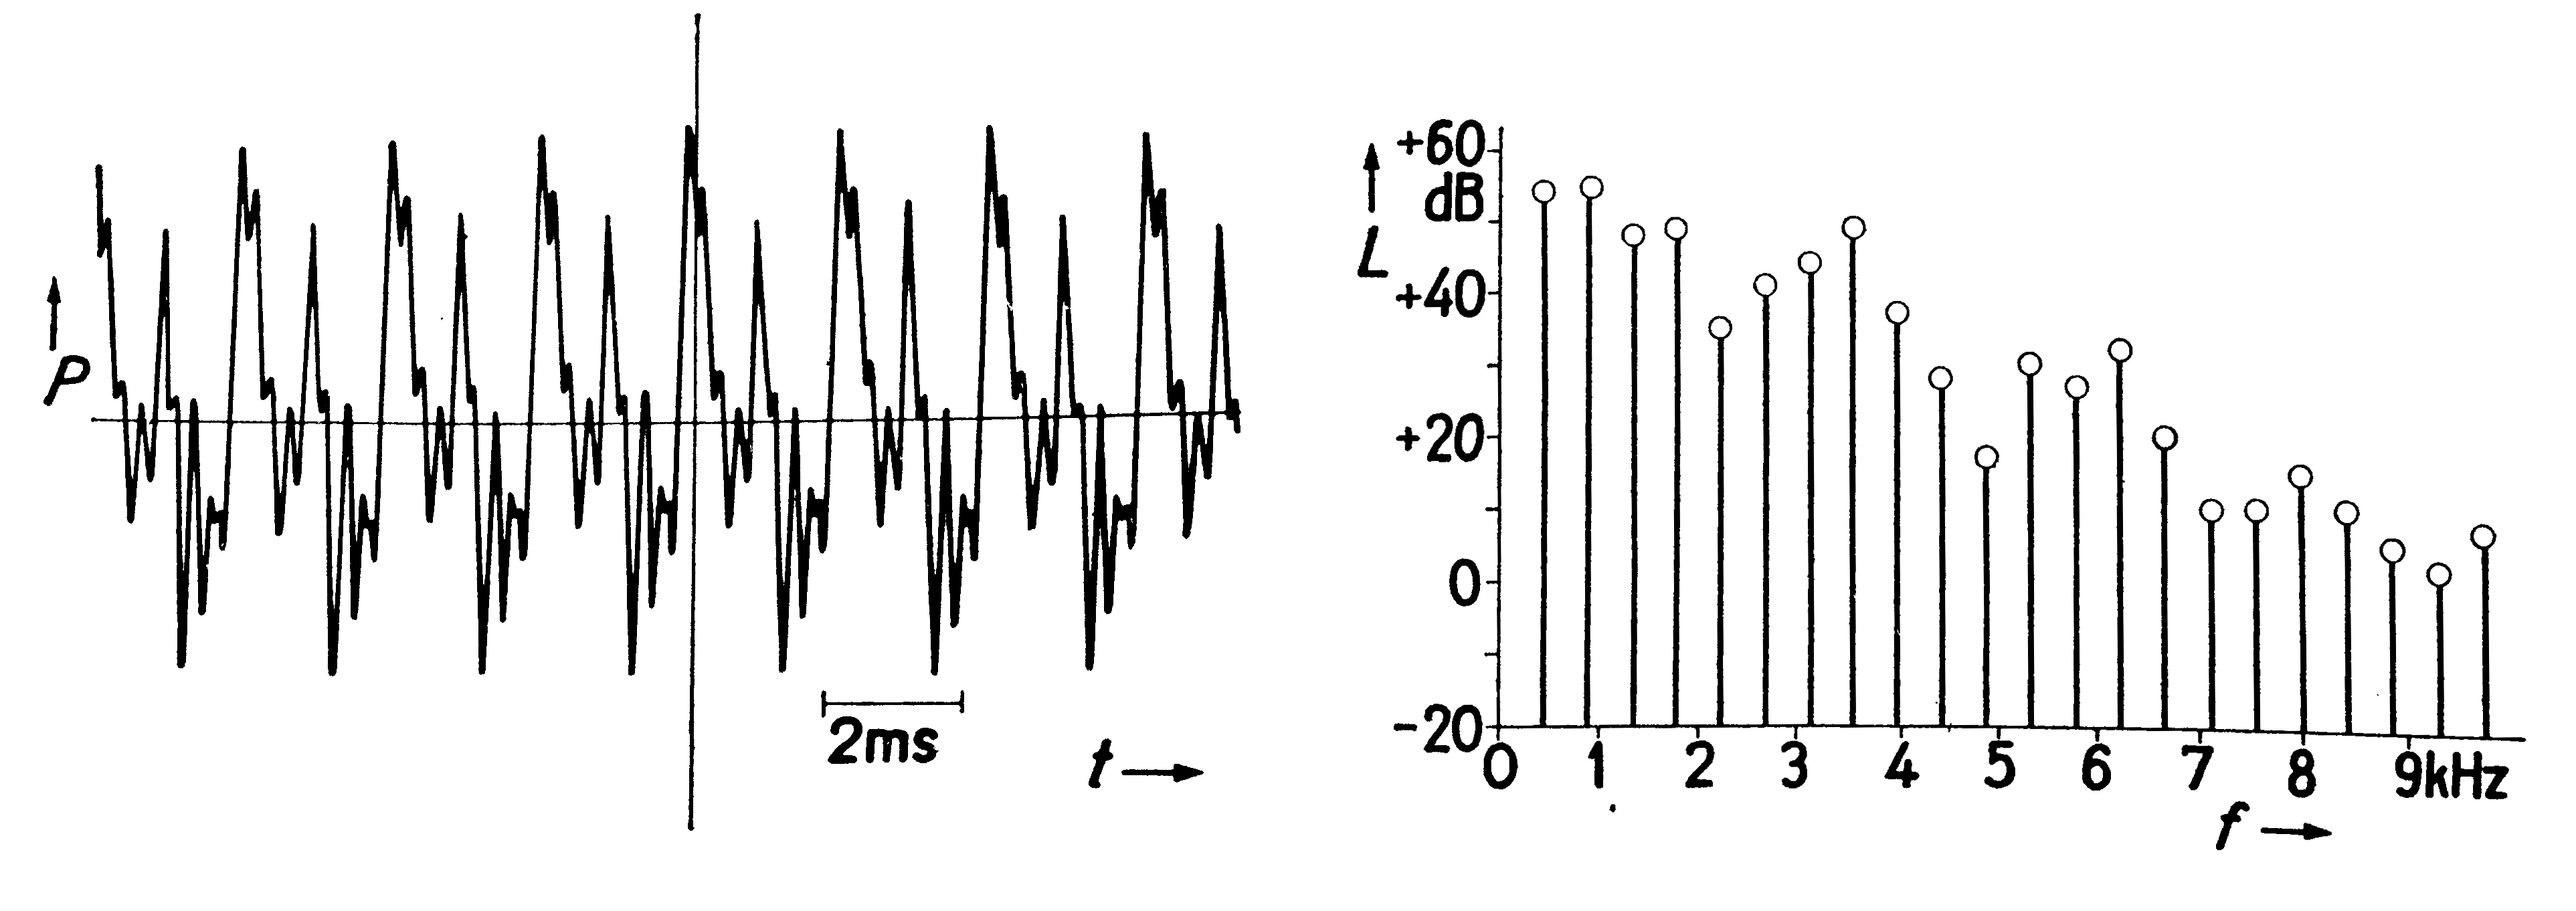
\includegraphics[width=0.95\textwidth]{GeigenTon.png}
\caption{Links: Schalldruck eines Geigenklangs; Rechts: Frequenzspektrum dieses Klanges}
\label{fig:geige}
Quelle: \cite[S. 4]{zwicker}
\end{figure}
\FloatBarrier

Um daher einen ungefähren Eindruck eines synthetisierten Tones zu bekommen, reicht es nicht aus, die berechnete Kurve (Wellenform) zu betrachten, welche eine Funktion der Zeit ist. Daher muss eine Alternative Darstellung des Signals gesucht werden. Ein \textbf{Frequenzspektrum} berechnet die Intensität einer gegeben Frequenz und ist somit eine Funktion der Frequenz. Das Frequenzspektrum lässt sich durch Fourier Analyse bestimmen. So kann jede komplexe Sinuswelle als Fourier Reihe dargestellt werden und somit als Addition aus mehreren Teilsinuswellen mit unterschiedlichen Amplituden. \cite[S. 33]{raichel} Durch mathematische Umformungen (siehe~\ref{matze:simplefm}), kann die Formel der FM-Synthese~\ref{eq:FM_Chowning} als folgende Summe dargestellt werden: \cite{chowningPaper}

% TODO siehe matze

\begin{equation}
\begin{split}
s(t)=A*\{\; & J_0(I)*\sin(\omega_c t)  \\
         +&J_1(I)*[\sin(t*(\omega_c + \;\,\omega_m))-\sin(t*(\omega_c-\;\,\omega_m))] \\
         +&J_2(I)*[\sin(t*(\omega_c + 2\omega_m))+\sin(t*(\omega_c-2\omega_m))] \\
         +&J_3(I)*[\sin(t*(\omega_c + 3\omega_m))-\sin(t*(\omega_c-3\omega_m))] \\
         +&....\}
\end{split}
\label{eq:chowningAddition}
\end{equation}

Hier bezieht sich $J_\nu(x)$ auf die Bessel Funktionen erster Ordnung. Bessel Funktionen zweiter Ordnung können dazu verwendet werden, Lösungen für nicht ganzzahlige $\nu$ Werte zu finden. Im Zusammenhang mit der FM-Synthese werden jedoch nur ganzzahlige $\nu$ Werte benötigt, daher genügt die Bessel Funktion erster Ordnung und $\nu$ wird mit $n$ angegeben. [TODO CITE; Temme] Abbildung~\ref{fig:bessel2D} stellt die ersten drei Bessel Funktionen dar.

\begin{figure} [ht]
\centering
  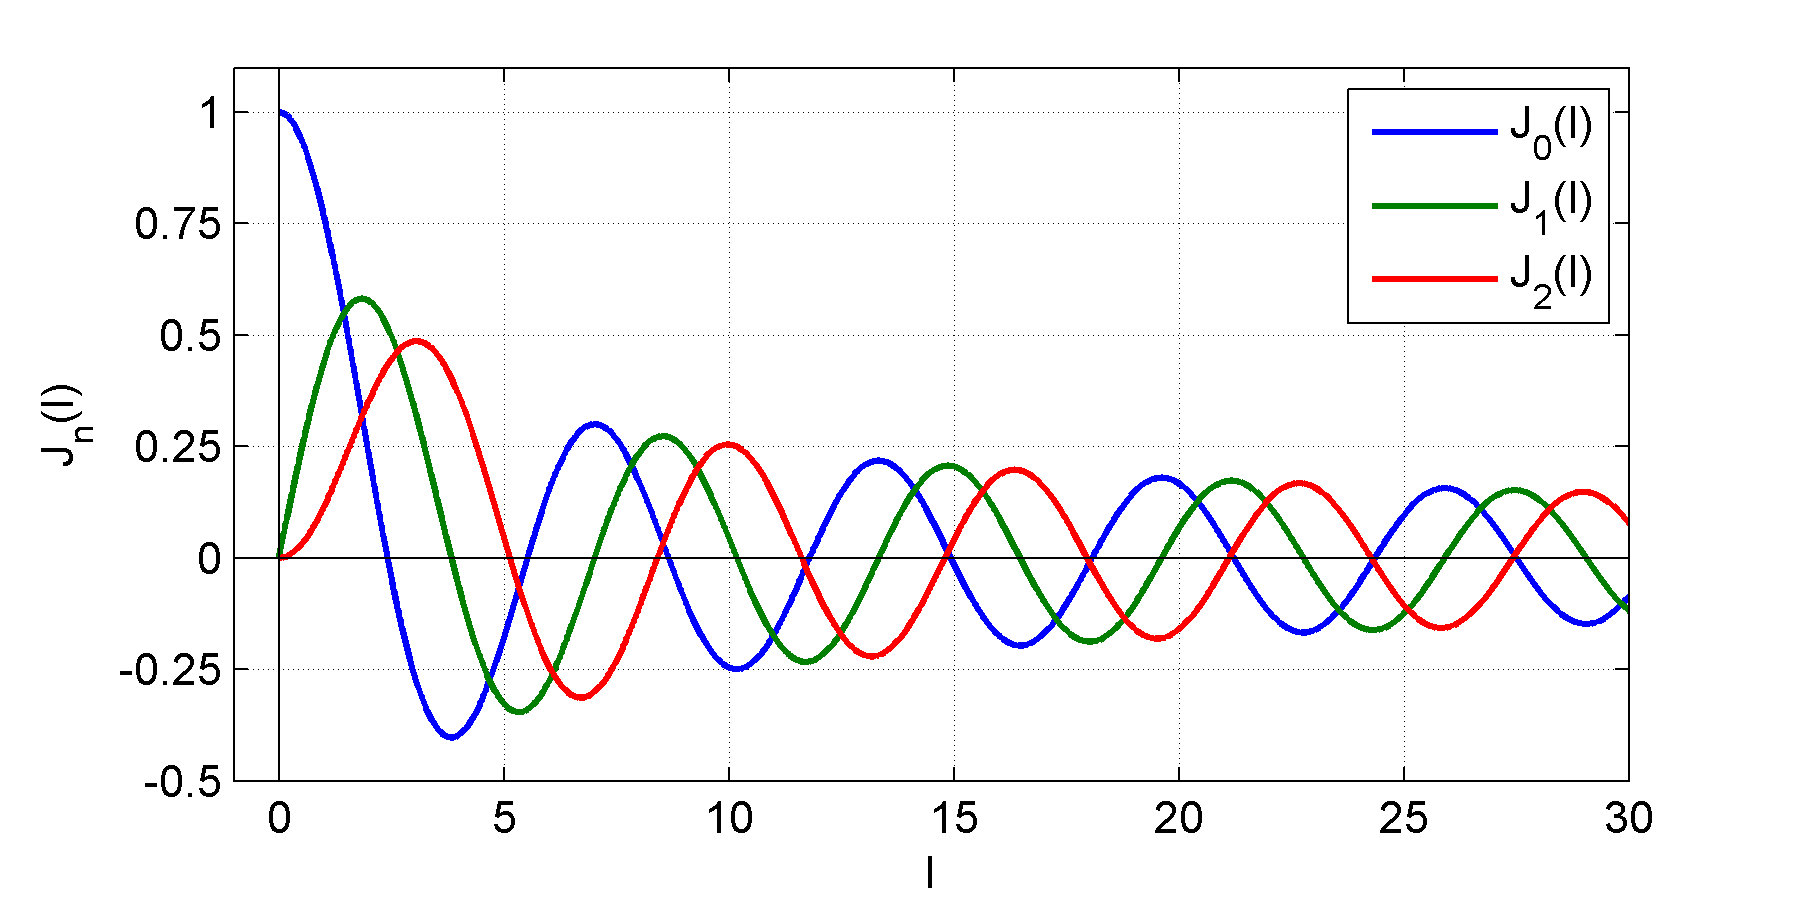
\includegraphics[width=0.80\textwidth]{Bessel2D.png}
\caption{2D-Plot der Bessel Funktionen $J_0$, $J_1$ und $J_2$.}
\label{fig:bessel2D}
Quelle: Eigene Darstellung mit MATLAB
\end{figure}

\FloatBarrier


Allgemein sind die Bessel Funktionen Lösungen für die Besselsche Differentialgleichung. Bei der FM-Synthese treten sie in Erscheinung, sobald die Formel~\ref{eq:FM_Chowning} der FM-Synthese als Fourier-Reihe dargestellt wird. Eine Fourier-Reihe setzt sich aus der Addition aus Sinus Funktionen multipliziert mit einem Fourier-Koeffizienten zusammen. Für die FM-Synthese entspricht dieser Koeffizient der Bessel Funktionen erster Ordnung. \cite[S. 221]{lathi} Die genaue mathematische Herleitung soll an dieser Stelle nicht behandelt werden. Es soll jedoch angemerkt sein, dass $J_n(x)$ nicht elementar berechnet werden kann und numerisch bestimmt werden muss. [TODO CITE] \cite[S. 385]{abramowitz} Funktionswerte können in geeigneten Tabellen nachgeschlagen werden. \cite{davis}
% aabramowitz s. 369??

Wie oben beschrieben, besteht ein Klang nicht nur aus seinem Grundton sondern auch aus Seitenfrequenzbänder. Theoretisch treten unendlich viele solcher Frequenzbänder auf, jedoch werden diese nicht mehr vom Ohr wahrgenommen, wenn sie eine gewisse Grenze an Intensität unterschreiten. Die Amplitude des Grundtones lässt sich durch $J_0(I)$ berechnen, wobei $I$ für den Modulationsindex steht. Dies lässt sich auch einfach aus Formel~\ref{eq:chowningAddition} entnehmen. Der erste Additionsterm $J_0(I)\sin(\omega_c t)$ entspricht der Trägerfrequenz. Bei einem Modulationsindex von $I=0$ findet keine Frequenzmodulation statt. An Abbildung~\ref{fig:bessel2D} wird ersichtlich, dass $J_0(0)=0$ ist. Für alle weiteren Bessel Funktionen gilt $J_n(0)=0$, damit reduziert sich die Addition aus Formel~ \ref{eq:chowningAddition} auf die Grundschwingung $1*sin(\omega_c t)$ und deckt sich somit mit unserer Erwartung, dass keine Modulation statt findet. Daraus lässt sich erschließen, dass die Trägerfrequenz $\omega_c$ dem Grundton entspricht.

\label{bulli:besselModIndexZusammenahang}
Wird nun der Modulationsindex stetig erhöht, wird Energie aus der Grundfrequenz genommen und auf die Seitenbänder verteilt. Dies lässt sich wieder an Abbildung~\ref{fig:bessel2D} erkennen. Wird $I$ größer, fällt die Amplitude von $J_0(I)$ ab und die restlichen Bessel Funktionen steigen an. $J_0(I)$ durchläuft den Nullpunkt bei $\approx2,5$, das bedeutet bei einem Modulationsindex von ungefähr $2,5$ ist der Grundton nicht im Frequenzspektrum vorhanden, sondern nur noch Seitenfrequenzen. In Abbildung~ \ref{fig:chowningEnergieVerteilung} wird der Modulationsindex von $0$ bis $4$ inkrementiert. Es wird ersichtlich, wie immer mehr Seitenfrequenzen entstehen und dabei die Grundfrequenz abnimmt. In Abbildung~ \ref{fig:chowningEnergieVerteilung} wird der Betrag der Amplitude dargestellt, somit wird die Grundfrequenz für $I=3$ im Vergleich zu $I=2$ wieder größer, da die Bessel Funktion den Nullpunkt durchlaufen hat und im negativen Bereich größer wird, bis das lokale Minimum erreicht wird und der Betrag wieder bis $0$ abnimmt.

\begin{figure} [ht]
\centering
  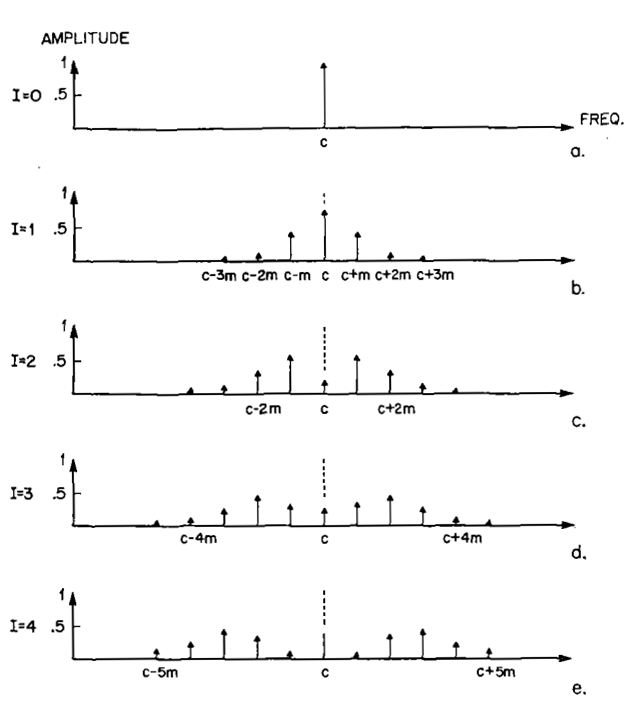
\includegraphics[width=0.5\textwidth]{Chowning_EnergieVerteilung.png}
\caption{Beispiel zur Veranschaulichung der zunehmender Bandbreite in Abhängigkeit eines wachsenden Modulationsindex. $c$ entspricht der Trägerfrequenz; $c\pm n*m$ entspricht der n-ten Seitenfrequenz.}
\label{fig:chowningEnergieVerteilung}
Quelle: \cite{chowningPaper}
\end{figure}
\FloatBarrier

An Abbildung~\ref{fig:chowningEnergieVerteilung} erkennt man auch, dass die Seitenfrequenzen sich symmetrisch in negativer und positiver Richtung zur Grundfrequenz ausbreiten. Dies erkennt man auch an Formel~\ref{eq:chowningAddition}, der innere Teil vom Sinus entspricht der Seitenfrequenz, wobei $(\omega_c+n*\omega_m)$ der n-ten Oberschwinung entspricht und $(\omega_c-n*\omega_m)$ der n-ten Unterschwinung. $J_n(I)$ gibt die Amplitude der n-ten Unter- und Oberschwinung an. 
Dies ist ein Vorteil der FM-Synthese im Vergleich zu anderen Sound Synthese Verfahren. Durch eine relativ simple Änderung des Modulationsindex können komplexe Klänge mit reichen Klangspektrum erzeugt werden.
Wie in Kapitel XX [TODO ref Julius] beschrieben, ist es jedoch schwer das Ergebnis der FM-Synthese vorher zusehen. Dies liegt zum einen an dem schwingenden Verlauf der Bessel Funktionen und deren Zusammenspiel.
Zum Anderen an zwei Effekten bei der Bestimmung des Frequenzspektrums, die in Abbildung~ \ref{fig:chowningEnergieVerteilung} ignoriert wurden, machen die Vorhersehbarkeit noch schwerer. Der erste Effekt betrifft negative Seitenfrequenzen. Deren Vorzeichen invertiert wird und somit, anschaulich, an der Ordinate in den positiven Frequenzbereich reflektiert werden. [TODO warum ist das so?] Der zweite Effekt betrifft Frequenzen, die den selben Wert haben. Dabei werden die Amplituden der gleichen Frequenzen algebraisch addiert. Dies kann auch zuvor reflektierte Frequenzen betreffen. Daher kann es unter Umständen schwer sein, einen gegeben Klang durch FM-Synthese zu rekonstruieren, da man keine direkte Kontrolle über die Teiltöne wie bei der additiven Synthese hat. Abbildung~\ref{fig:chowningFreqReflektion} veranschaulicht das Verhalten der Seitenfrequenzen. Als einfaches Beispiel wählte Chowning $\omega_c=\omega_m=100$ und $I=4$.


\begin{figure} [ht]
\centering
  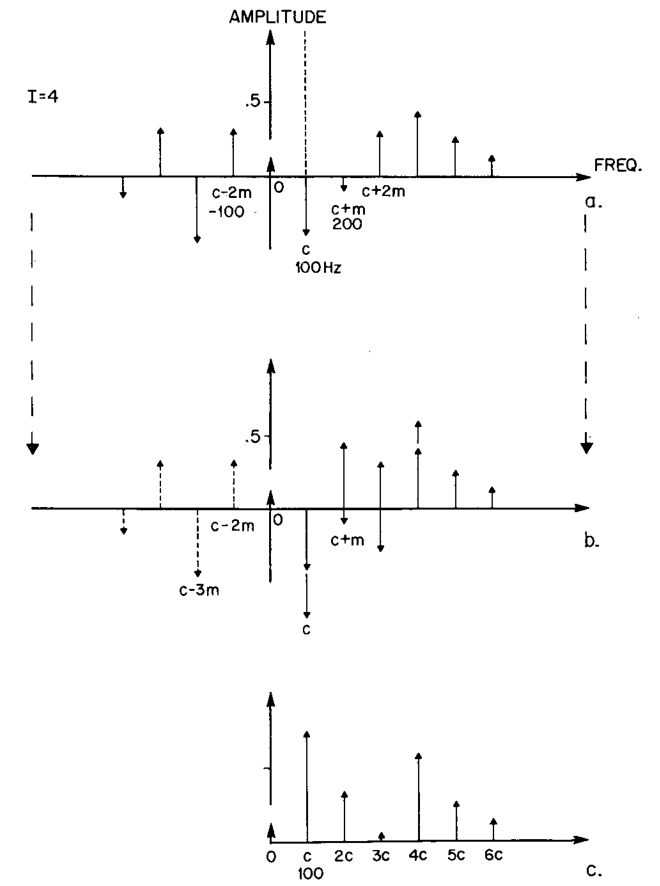
\includegraphics[width=0.5\textwidth]{ChowningFreqReflektion.png}
\caption{TODO}
\label{fig:chowningFreqReflektion}
Quelle: \cite{chowningPaper}
\end{figure}
\FloatBarrier





\begin{figure} [ht]
\centering
  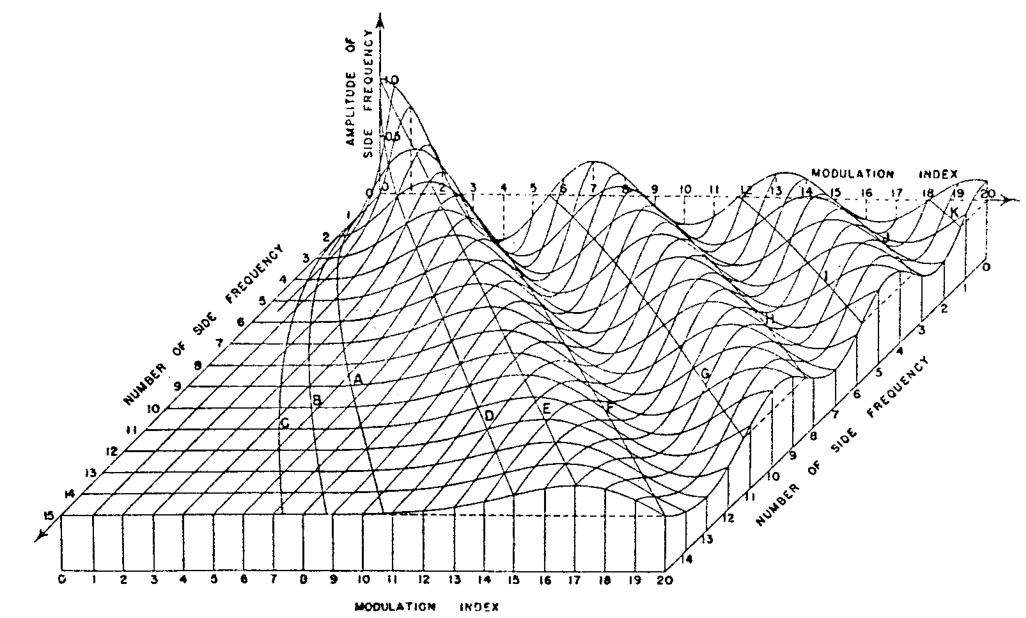
\includegraphics[width=0.95\textwidth]{ChowningBessel.png}
\caption{Besselfunktion $J_0$ bis $J_{15}$ und Modulationsindex $I$ von 0 bis 20. }
\label{fig:bessel3D}
Quelle: \cite{chowningPaper}
\end{figure}



Durch die zeitliche Änderung der Frequenz bei der Frequenzmodulation entstehen Seitenfrequenzbänder.


Das Frequenzspektrum eines natürlichen Tons ist selten statisch sondern variiert mit der Zeit. Diese Änderung der Teiltöne lässt das menschliche Ohr Töne unterschiedlich wahrnehmen. Durch die FM-Synthese lassen sich, im Vergleich zu anderen Syntheseverfahren, auf einfachen Weg komplexe und vielfältige Frequenzspektren künstlich erzeugen.

\FloatBarrier
\subsubsection{Harmonische Frequenzverhältnisse(Inkl. Vibrato)}


\FloatBarrier